%9T5 
\setcounter{paragraph}{0}
\PhanI
\loai{Tìm số cực tiểu trên đoạn hai nguồn}
\begin{ex}%[3P2B6-1][Loai1]
Tại hai điểm A và B hai nguồn sóng kết hợp cách nhau 10 cm trên mặt nước dao động cùng pha với nhau. Tần số dao động là 40 Hz. Tốc độ truyền sóng trên mặt nước là 80 cm/s. Số điểm dao động với biên độ cực tiểu trên đoạn AB là
\choice
{9}
{11}
{\True 10}
{12}
\loigiai{
\begin{itemize}
%\item Ta có: $\lambda = \dfrac{v}{f} = \dfrac{80}{40} = 2\ cm $.
\item Các điểm dao động với biên độ cực tiểu thỏa mãn:
\begin{align*}
-AB < (k + 0,5)\lambda < AB\ \ct{hay}\ -10 < (k + 0,5).2 < 10 \Rightarrow -5,5 < k < 4,5.
\end{align*}
%\item Vậy có 10 giá trị của k hay có 10 điểm dao động với biên độ cực tiểu trên đoạn AB.
\end{itemize}
}
\end{ex} \haidong{20}
\loai{Tìm số cực đại, cực tiểu trên đoạn thẳng có 1 đầu thuộc đường trung trực}
\begin{ex}%[3P2K6-1][Loai1]
Trong một thí nghiệm về giao thoa sóng trên mặt nước, hai nguồn kết hợp A và B dao động với cùng tần số $f=50$ Hz, cùng biên độ và cùng pha ban đầu. Tại một điểm M cách hai nguồn sóng đó những khoảng lần lượt là $d_1=42$ cm và $d_2=50$ cm, sóng có biên độ cực đại. Biết vận tốc truyền sóng trên mặt nước là 80 cm/s. Số đường cực đại giao thoa nằm trong khoảng M và đường trung trực của hai nguồn (không tính đường qua M) là
\choice
{3 đường}
{2 đường}
{\True 4 đường}
{5 đường}
\loigiai{
\begin{itemize}
\item Bước sóng: $\lambda = \dfrac{v}{f} = 1,6\ cm $.
\item Dễ thấy $d_1-d_2 = -8 = -5.\lambda \Rightarrow$ M là cực đại bậc 5.
\item Trong khoảng giữa M và đường trung trực của hai nguồn có 4 đường cực đại nữa.
\item 
\item 
\end{itemize}
}
\end{ex} \haidong{20}
 
\loai{Tìm số cực đại, cực tiểu trên đường chéo hình vuông}
\begin{ex}%[3P2K6-1][Loai1]
Ở mặt thoáng của một chất lỏng có hai nguồn sóng kết hợp A và B cách nhau 20 cm, dao động theo phương thẳng đứng với phương trình $u_A = u_B = 2\cos(40\pi t)$ ($u_A$ và $u_B$ tính bằng mm, t tính bằng s). Biết tốc độ truyền sóng trên mặt chất lỏng là 30 cm/s. Xét hình vuông AMNB thuộc mặt thoáng chất lỏng. Số điểm dao động với biên độ cực đại trên đoạn BM là
\choice
{\True 19}
{18}
{20}
{17}
\loigiai{
\immini{\begin{itemize}
\item $MB=AB\sqrt{2}=20\sqrt{2}\ cm$.
\item Số điểm dao động với biên độ cực đại trên đoạn MB là nghiệm bất phương trình: 
\begin{align*}
MA-MB<k_{cd}\lambda \le BA-BB\Leftrightarrow -5,52<k_{cd}\le 13,33.
\end{align*} 
\item Có 19 điểm cần tìm.
\end{itemize}}{
\begin{tikzpicture}[scale=1]
\tkzDefPoints{0/0/a, 3/0/b, 3/3/n, 0/3/m}
\tkzDrawSegments(a,b b,n n,m a,m b,m)
\tkzLabelPoint[below](a){$A$}
\tkzLabelPoint[above](m){$M$}
\tkzLabelPoint[above](n){$N$}
\tkzLabelPoint[below](b){$B$}
\tkzDrawPoints[size=3,fill=white](a,b,m,n)
\end{tikzpicture}}
}\end{ex} \haidong{20}

\loai{Tìm số cực đại, cực tiểu trên một cạnh của tam giác}
\begin{ex}%[3P2K6-1][Loai1]
Ba điểm A, B, C trên mặt nước là ba đỉnh của một tam giác vuông ở A, trong đó A và B là hai nguồn sóng nước giống nhau, cách nhau 8 cm, cùng phát sóng có bước sóng là 3,2 cm. Khoảng cách $AC = 8,4$ cm thì số điểm dao động với biên độ cực đại có trên đoạn AC là
\choice
{4}
{5}
{3}
{\True 2}
\loigiai{
\begin{itemize}
\item $\Delta ABC$ vuông tại A $\Rightarrow  CB=\sqrt{AB^2+AC^2}=11,6\ cm$.
\item Số điểm dao động với biên độ cực đại trên đoạn AC là nghiệm bất phương trình:
\begin{align*}
AA-AB<k_{cd}\lambda \le CA-CB\Leftrightarrow -8<3,2k_{cd}\le -3,2\Leftrightarrow -2,5<k_{cd}\le -1\Rightarrow k_{cd}=-2;\ -1.
\end{align*} 
\item Có 2 điểm cần tìm.
\item 
\item 
\end{itemize}
}
\end{ex} \haidong{20}
\loai{Tìm số cực đại, cực tiểu trên đường vuông góc với đoạn hai nguồn tại nguồn}
\begin{ex}%[3P2K6-1][Loai1]
Trong hiện tượng giao thoa sóng nước hai nguồn kếp hợp A và B cách nhau 25 cm dao động với phương trình: $u_A=u_B=3\cos(40\pi t)$ cm. Biết tốc độ truyền sóng trên mặt nước $v=0,4$ m/s. Gọi d là đường thẳng thuộc mặt nước đi qua A và vuông góc với AB. Số điểm dao động với biên độ cực đại trên đường thẳng d là
\choice
{\True 24}
{26}
{23}
{25}
\loigiai{
\begin{itemize}
\item Ta có: $\lambda = \dfrac{v}{f} = \dfrac{40}{20} = 2$ cm.
\item Số vân cực đại trên AB $\dfrac{-AB}{\lambda } < k < \dfrac{AB}{\lambda } \Rightarrow \dfrac{-25}{2} < k < \dfrac{25}{2} \Rightarrow -12,5 < k < 12,5$.
\item Các vân cực đại nằm trong vùng từ vân trung tâm đến nguồn A thì cắt được d $\Rightarrow$ có 12 vân cực đại thỏa mãn.
\item Mỗi vân cực đại cắt d tại hai điểm $\Rightarrow$ có $12.2=24$ điểm dao động với biên độ cực đại. 
\item 
\item 
\item 
\end{itemize}
}
\end{ex} \haidong{20}
\loai{Tìm số cực đại, cực tiểu trên đoạn thẳng nằm trên đoạn hai nguồn}
\begin{ex}%[3P2K6-1][Loai1]
Tại hai điểm A và B trên mặt chất lỏng có hai nguồn phát sóng kết hợp cùng phương, cùng pha và tạo ra sóng với bước sóng $\lambda$. Khoảng cách AB bằng $4,5\lambda$. Gọi E, F là hai điểm trên đoạn AB sao cho $AE=EF=FB$. Số cực đại, cực tiểu trên đoạn EF lần lượt là
\choice
{2 và 3}
{3 và 2}
{4 và 3}
{\True 3 và 4}
\loigiai{
\begin{center}
\begin{tikzpicture}[scale=1]
\tkzDefPoints{0/0/a, 3/0/e, 6/0/f, 9/0/b}
\tkzDrawSegments(a,b)
\tkzDrawPoints[size=3,fill=black](a,e,f,b)
\tkzLabelSegment(a,e){$1,5\lambda$}
\tkzLabelSegment(e,f){$1,5\lambda$}
\tkzLabelSegment(f,b){$1,5\lambda$}
\tkzLabelPoint[below](a){$A$}
\tkzLabelPoint[below](e){$E$}
\tkzLabelPoint[below](f){$F$}
\tkzLabelPoint[below](b){$B$}
\end{tikzpicture}
\end{center}
\begin{align*}
\begin{cases}
k_E=\dfrac{\left(d_{1E}-d_{2E}\right)}{\lambda}=\dfrac{\left(1,5\lambda -3\lambda\right)}{\lambda}=-1,5\\
k_F=\dfrac{\left(d_{1F}-d_{2F}\right)}{\lambda}=\dfrac{\left(3\lambda -1,5\lambda\right)}{\lambda}=1,5\\
\end{cases} \Rightarrow
\begin{cases}
\text{Số cực đại}:-1,5\le k\le 1,5\Rightarrow k=\underbrace{-1;0;1}_{\text{có 3 cực đại}}\\
\text{Số cực tiểu}:-1,5\le m-0,5\le 1,5\Rightarrow m=\underbrace{-1;0;1;2}_{\text{có 4 cực tiểu}}\\
\end{cases}
\end{align*}
}
\end{ex} \haidong{20}
\loai{Tìm số cực đại, cực tiểu trên đường tròn bao cả hai nguồn bên trong}
\begin{ex}%[3P2K6-1][Loai1]
Ở mặt nước có hai nguồn sóng cơ A và B cách nhau 16 cm, dao động điều hòa cùng tần số, cùng pha theo phương vuông góc với mặt nước. Điểm M nằm trên AB, cách trung điểm O là 1,5 cm, là điểm gần O nhất luôn dao động với biên độ cực đại. Trên đường tròn tâm O, đường kính 20 cm, nằm ở mặt nước có số điểm luôn dao động với biên độ cực đại là
\choice
{18}
{16}
{\True 22}
{17}
\loigiai{
\begin{itemize}
\item Hai nguồn cùng pha nên trung điểm hai nguồn là một cực đại, M cách O gần nhấ là 1,5 dao động với biên độ cực đại nên $\lambda = 3\ cm $.
\item Hai nguồn dao động cùng pha nên số điểm dao động với biên độ cực đại trên đường nối hai nguồn ứng với giá trị: $\dfrac{-AB}{\lambda} \leq k \leq \dfrac{AB}{\lambda} \Leftrightarrow-5,3 \leq k \leq 5,3   \Rightarrow$ có 11 giá trị.
\item Do đường kính của đường tròn tâm O là 20 $\Rightarrow$ hai nguồn nằm trong đường tròn nên số điểm dao động với biên độ cực đại trên đường tròn là: $2.11=22$ điểm.

\end{itemize}
}
\end{ex} \haidong{20}
\loai{Tìm số cực đại, cực tiểu trên đường tròn đường kính nhỏ hơn đoạn hai nguồn}
\begin{ex}%[3P2K6-1][Loai1]
Trong thí nghiệm giao thoa của sóng nước, khoảng cách giữa hai mũi nhọn gắn với cần rung là $S_1S_2 = 12,5$ cm. Tốc độ truyền sóng là 150 cm/s. Tần số dao động của cần rung 75 Hz. Trên mặt nước lấy đường tròn tâm O là trung điểm của $S_1S_2$ có bán kính 4,0 cm. Số điểm dao động với biên độ cực tiểu trên đường tròn là
\choice
{24}
{20}
{18}
{\True 16}
\loigiai{
\begin{itemize}
\item  Số điểm dao động cực tiểu trên đường kính MN: 
\begin{align*}
MA-MB\le \left(k_{ct}-0,5 \right)\lambda \le NA-NB\Leftrightarrow -3,5\le {{k}_{ct}}\le 4,5.
\end{align*}
$\Rightarrow$  Có 8 dãy cực tiểu cắt MN, trong đó không có dãy nào đi qua 2 mút M và N. 
\item Mỗi dãy cắt đường tròn tại 2 điểm
$\Rightarrow$ trên đường tròn có 16 điểm dao động với biên độ cực tiểu.

\end{itemize}
}
\end{ex} \haidong{20}

\loai{Loại khác}
\begin{ex}%[3P2K6-1][Loai1]
Ở mặt thoáng của một chất lỏng có hai nguồn sóng kết hợp A và B cách nhau 20 cm, dao động theo phương thẳng đứng với phương trình $u_A=u_B=4\cos(40\pi t)$ cm. Biết tốc độ truyền sóng trên mặt chất lỏng là 40 cm/s. Xét hình thoi BMNA có $AB=BN$ thuộc mặt thoáng chất lỏng. Số điểm dao động với biên độ cực đại trên đoạn AM là
\choice
{19 điểm}
{18 điểm}
{\True 17 điểm}
{16 điểm}
\loigiai{
\begin{itemize}
\item ABMN là hình thoi có AB=BN $\Rightarrow \widehat{ABM} = 120\degree \Rightarrow AM = AB\sqrt{3} = 20\sqrt{3}\ cm$.
\item Ta có: $\lambda = \dfrac{v}{f} = 2\ cm$.
\item Điều kiện để một điểm dao động với biên độ cực đại: 
\begin{align*}
d_1-d_2 = k.\lambda = 2k\Rightarrow 0-20 < 2k < 20\sqrt{3}-20\Rightarrow -10 < k < 7,32.
\end{align*}
\item Có 17 điểm dao động với biên độ cực đại trên AM. 

\end{itemize}
}
\end{ex} \haidong{20}
\begin{ex} %[3P2G6-1][Loai1]
Ở mặt thoáng của một chất lỏng có hai nguồn sóng kết hợp A và B cách nhau 20 cm, dao động theo phương thẳng đứng với phương trình $u_A = u_B = 2\cos(40\pi t )$ ($u_A$ và $u_B$ tính bằng mm, t tính bằng s). Biết tốc độ truyền sóng trên mặt chất lỏng là 30 cm/s. Xét hình vuông AMNB thuộc mặt thoáng chất lỏng. Số điểm dao động với biên độ cực đại trên chu vi hình vuông AMNB là
\choice
{56}
{58}
{\True 54}
{62}
\loigiai{
\begin{itemize}
\item $MB=AB\sqrt{2}=20\sqrt{2}\ cm$.
\item Số điểm dao động với biên độ cực đại trên đoạn AB là $2.\left[ \dfrac{AB}{\lambda } \right]+1=27$.
\item Số điểm dao động với biên độ cực đại trên đoạn AM là nghiệm bất phương trình:
\begin{align*}
AA-AB<k_{cd}\lambda \le MA-MB\Leftrightarrow -13,33<k_{cd}\le -5,52   \Rightarrow\ \ct{có 8 điểm}.
\end{align*}
\item Theo tính chất đối xứng thì số điểm dao động với biên độ cực đại trên NB giống với trên AM, tức 8 điểm.
\item Số điểm dao động với biên độ cực đại trên đoạn MN là nghiệm bất phương trình:
\begin{align*}
MA-MB\le k_{cd}\lambda \le NA-NB\Leftrightarrow -5,52\le k_{cd}\le 5,52   \Rightarrow\ \ct{có 11 điểm}.
\end{align*}
\item Vậy tổng có $27 + 8.2 + 11 = 54$ điểm cần tìm.

\end{itemize}
}
\end{ex} \haidong{20}






























%macbook 
\loai{Vị trí cực tiểu trên đoạn hai nguồn}
\begin{ex}%[3P2K6-2][Loai1]
Trên bề mặt chất lỏng có hai nguồn A và B đồng bộ cách nhau 4,5 cm. Bước sóng lan truyền 1,2 cm. Điểm cực tiểu trên khoảng OB cách O (O là trung điểm) gần nhất và xa nhất lần lượt là
\choice
{\True 0,3 cm và 2,1 cm}
{0,6 cm và 1,8 cm}
{1 cm và 2 cm}
{0,2 cm và 2 cm}
\loigiai{
\begin{itemize}
\item Hai nguồn kết hợp cùng pha (O là cực đại), cực tiểu thuộc OB:
$x=m\dfrac{\lambda}{2}+\dfrac{\lambda}{4}\begin{cases}
x_{\min}=\dfrac{\lambda}{4}=0,3\ cm.\\
x_{\max}=n\dfrac{\lambda}{2}+\dfrac{\lambda}{4}.\\
\end{cases}$
\item Với n là số nguyên lớn nhất thỏa mãn
$n<\dfrac{OB-x_{\min}}{0,5\lambda}=\dfrac{\dfrac{4,5}{2}-0,3}{0,5.1,2}=3,25\Rightarrow n=3$
$\Rightarrow x_{\max}=n\dfrac{\lambda}{2}+\dfrac{\lambda}{4}=2,1\ cm$.
\end{itemize}
}
\end{ex} \haidong{20}
\loai{Vị trí cực đại xa nhất trên đường vuông góc với đoạn hai nguồn tại nguồn}
\begin{ex}%[3P2K6-2][Loai1]
Trong hiện tượng giao thoa sóng nước, hai nguồn dao động theo phương vuông góc với mặt nước, cùng biên độ, cùng pha, cùng tần số 25 Hz được đặt tại hai điểm A và B cách nhau 10 cm. Tốc độ truyền sóng trên mặt nước là 40 cm/s. Xét các điểm trên mặt nước thuộc đường thẳng vuông góc với AB tại B, điểm mà phần tử tại đó dao động với biên độ cực đại cách điểm B một đoạn lớn nhất bằng
\choice
{32,05 cm}
{\True 30,45 cm}
{0,41 cm}
{10,01 cm}
\loigiai{
\immini{\begin{itemize}
\item Vẽ hình, thấy rằng điểm M cần tìm thuộc dãy cực đại $k_{cd} = 1\Rightarrow MA - MB = 1.\lambda$.
\item Mà $MA^2 - MB^2 = AB^2\Rightarrow 2.MB = \dfrac{AB^2}{1.\lambda }-1.\lambda  \Rightarrow MB = 30,45$ cm.
\end{itemize}}{\begin{tikzpicture}[scale=1]
\begin{scope}[shift={(0,0)}]
\tkzInit[ymin=-2,ymax=2,xmin=-1.5,xmax=2]\tkzClip
\tkzDefPoints{0/0/o, -1/0/s1, 1/0/s2, 1/1.75/m, 1/1.35/n, 1/0.26/k}
\draw[red] plot[domain=-0.9:0.9] ({0.8*cosh(\x)},{0.35*sinh(\x)});
\draw[red] plot[domain=-1.7:1.7] ({0.25*cosh(1.3*\x)},{0.58*sinh(\x)});
\draw[red] plot[domain=-4:4, samples=100] ({0.125*cosh(1.5*\x)},{0.57*sinh(\x)});
\draw[red](0,3)--(0,-3);
\draw[blue](1,3)--(1,-3);
\draw[blue](s1)--(s2);
\draw[blue](s1)--(m);
\tkzLabelPoint[left](s1){$A$}
\tkzLabelPoint[right](s2){$B$}
\tkzDrawPoints[size=3,fill=white](m,n,s1,s2,k,o)
\tkzLabelPoint[left](m){$M$}
\tkzLabelPoint[below left](o){$O$}
\tkzLabelPoint[right](m){$1$}
\tkzLabelPoint[right](n){$2$}
\tkzLabelPoint[above right](k){$k_{max}$}
\end{scope}
\end{tikzpicture}}
}
\end{ex} \haidong{20}
\loai{Vị trí cực tiểu trên đường vuông góc với đoạn hai nguồn tại nguồn}
\begin{ex}%[3P2K6-2][Loai1]
Tại hai điểm A và B trên mặt chất lỏng có hai nguồn phát sóng cơ cùng pha cách nhau $AB = 8\ cm$, dao động với tần số 20 Hz. Một điểm M trên mặt nước, cách A một khoảng 25 cm và cách B một khoảng 20,5 cm, dao động với biên độ cực đại. Giữa M và đường trung trực của AB có hai vân giao thoa cực đại. Coi biên độ sóng truyền đi không giảm. Điểm Q thuộc đường thẳng vuông góc với AB tại A. Điểm Q dao động với biên độ cực tiểu cách A lớn nhất một đoạn bao nhiêu?
\choice
{\True 42,3 cm}
{20,6 cm}
{1,4 cm}
{0,5 cm}
\loigiai{
\begin{itemize}
\item M dao động với biên độ cực đại, giữa M và trung trực còn 2 dãy cực đại $\Rightarrow$ M thuộc dãy cực đại thứ 3
$\Rightarrow MA - MB = 3\lambda \Rightarrow \lambda = 1,5$ cm.
\item Vẽ hình và dễ thấy rằng điểm Q cần tìm thuộc dãy cực tiểu $k_{ct} = 1$\\
$\Rightarrow QB - QA = 0,5.\lambda$. 
\item Mà $ QB_2 - QA_2 = AB_2\Rightarrow 2.QA = \dfrac{AB^2}{0,5.\lambda }-0,5.\lambda  \Rightarrow QA = 42,3$ cm.
\item 
\item 
\item 
\end{itemize}
}
\end{ex} \haidong{20}
\loai{Vị trí cực đại trên đường tròn đường kính là đoạn hai nguồn}
\begin{ex}%[3P2K6-2][Loai1]
Trên mặt nước có hai nguồn kết hợp A, B dao động cùng pha và cách nhau 8 cm, bước sóng do sóng từ các nguồn phát ra là 3 cm. Điểm M dao động với biên độ cực đại trên đường tròn đường kính AB cách A xa nhất một khoảng là
\choice
{7,9 cm}
{\True 7,8 cm}
{6,7 cm}
{7,6 cm}
\loigiai{
\immini{\begin{itemize}
\item Rõ ràng M thuộc dãy cực tiểu ngoài cùng (phía B) $k_{cd}(max) =  \left[ \dfrac{AB}{\lambda } \right]= 2$\\
$\Rightarrow MA - MB = 2.\lambda = 6$ cm $\Rightarrow MB = MA - 6\quad (*)$
\item Mà $\Delta AMB$ vuông tại M $\Rightarrow MA^2+MB^2=AB^2=8^2$.
\item Thế vào $(*) \Rightarrow 2MA^2 - 12MA - 28 = 0 \Rightarrow MA = 7,8\ cm$.
\end{itemize}}{\begin{tikzpicture}[scale=0.6,thick,>=stealth']
\tkzDefPoints{0/0/a, 3/0/o, 6/0/b, 3/4/p, 3/-4/q, 5/4/y, 5/-4/y'}
\tkzDefShiftPoint[o](63:3){m}
\tkzDrawCircle[radius](o,a)
\tkzDrawSegments[dashed](p,q a,b a,m b,m)
\tkzDrawPoints[size=3](a,b,o,m)
\tkzMarkRightAngles(a,m,b)
\draw[blue](y) to [bend right =30](y');
\node at (a)[below left]{$A$};
\node at (b)[below right]{$B$};
\node at (m)[above right]{$M$};
\node at (o)[below left]{$O$};
\end{tikzpicture}}
}
\end{ex} \haidong{20}
\loai{Vị trí cực đại xa (gần) trung trực nhất trên đường tròn bán kính là đoạn hai nguồn}

\begin{ex}%[3P2G6-2][Loai1]
Trên mặt nước, hai nguồn kết hợp A, B cách nhau 20 cm dao động điều hòa cùng pha, tạo ra sóng có bước sóng 3 cm. Xét các điểm trên mặt nước thuộc đường tròn tâm A, bán kính AB, điểm nằm trên đường tròn dao động với biên độ cực đại cách xa đường trung trực của AB nhất một khoảng bằng
\choice
{34,5 cm}
{\True 26,1 cm}
{21,7 cm}
{19,7 cm}
\loigiai{
\immini{\begin{itemize}
\item $\text{số nguyên lớn nhất}<\dfrac{AB}{\lambda}=\dfrac{20}{3}=6,7\Rightarrow n=6$.
\item Điểm M phải là cực đại gần A nhất nên:\\ $MA-MB=-6\lambda \Rightarrow MB=38\ cm$.
\item $\cos \alpha =\dfrac{AB^2+MB^2-MA^2}{2.AB.MB}=0,95$.
\end{itemize}}{\begin{tikzpicture}[scale=0.7,thick,>=stealth']
\tkzInit[ymin=-4,ymax=4,xmin=-3.5,xmax=4]\tkzClip
\tkzDefPoints{0/0/a, 1.5/0/o, 3/0/b, 1.5/3.5/p, 1.5/-3.5/q, -0.5/3/y, -0.5/-3/y', -3/0/b'}
\tkzDefShiftPoint[a](100:3){m}
\tkzDefShiftPoint[a](-100:3){n}
\tkzDefPointBy[projection=onto p--q](m) \tkzGetPoint{i}
\tkzDefPointBy[projection=onto b--b'](m) \tkzGetPoint{h}
\tkzDrawCircle[radius](a,b)
\tkzDrawSegments(b',b b,m)
\tkzDrawSegments[dashed](h,m i,m p,q)
\tkzDrawPoints[size=3](a,b,o,m,n)
\tkzMarkAngles[size=0.5cm](m,b,b')
\tkzLabelAngle[pos=0.8](m,b,b'){$\alpha$}
\draw[blue](y) to [bend left =30](y');
\node at (a)[below]{$A$};
\node at (h)[below]{$H$};
\node at (i)[right]{$I$};
\node at (b)[below right]{$B$};
\node at (m)[above right]{$M$};
\node at (o)[below left]{$O$};
\end{tikzpicture}}}
\end{ex} \haidong{20}
\loai{Vị trí cực tiểu trên đường tròn bán kính là đoạn hai nguồn}
\begin{ex}%[3P2K6-2][Loai1]
Trong hiện tượng giao thoa sóng nước, hai nguồn A, B cách nhau 20 cm dao động cùng biên độ, cùng pha, cùng tần số 50 Hz. Tốc độ truyền sóng trên mặt nước là 1,5 m/s. Xét các điểm trên mặt nước thuộc đường tròn tâm A, bán kính AB, dao động với biên độ cực tiểu cách đường thẳng AB một đoạn ngắn nhất bằng
\choice
{18,67 mm}
{4,9675 mm}
{5,975 mm}
{\True 4,9996 mm}
\loigiai{
\immini{\begin{itemize}
\item Ta có: $\lambda = \dfrac{v}{f} = 3\ cm $.
\item Điều kiện để một điểm dao động với biên độ cực tiểu là\\
$-S_1S_2 \leq (k + 0,5)\lambda \leq S_1S_2$ hay $-20 \leq 3(k + 0,5) \leq 20 \Rightarrow -7,17 \leq k \leq 6,17$.
\item Để M cách AB một đoạn ngắn nhất thì M phải nằm trên cực tiểu thứ 7 $(k=6)\Rightarrow d_1-d_2 = (6 + 0,5).3 = 19,5$ cm.
\item Mà $ d_1 = 20\ cm \Rightarrow d_2 = 0,5\ cm $.
\item Ta lại có:
$d_1^2-(10 + x)^2 = d_2^2-(10-x)^2$ hay $20^2-(10 + x)^2 = 0,5^2-(10-x)^2\Rightarrow x=9,99375$ cm.
\item $\Rightarrow$ Khoảng cách từ M đến AB là $\sqrt{20^2-(10 + 9,99375)^2} = 0,49996\ cm = 4,9996\ mm.$
\end{itemize}}{\begin{tikzpicture}[scale=1,thick,>=stealth']
\tkzDefPoints{0/0/s1, 1/0/i, 2/0/s2, 1/3/y, 1/-3/y', 2.4/3/c, 2.4/-3/d}
\tkzDrawCircle[radius](s1,s2)
\tkzDefShiftPoint[s1](34:2){m}
\tkzDefPointBy[projection=onto s1--s2](m) \tkzGetPoint{h}
\tkzDrawSegments(s1,s2 m,h s1,m s2,m)
\tkzDrawSegments[red](y,y')
\tkzDrawPoints[size=3](s1,s2,i,m,h)
\draw[blue,dashed](c) to [bend right =30](d);
\draw [decorate,red,decoration={brace,mirror,amplitude=3pt},xshift=0pt,yshift=-4pt]
(h) -- (i) node [black,midway,yshift=10pt] 
{$x$};
\tkzLabelSegment[above](s1,m){$d_1$}
\tkzLabelSegment[right](s2,m){$d_2$}
\node at (s1)[below left]{$A$};
\node at (s2)[below right]{$B$};
\node at (i)[below left]{$I$};
\node at (m)[right]{$M$};
\node at (h)[below]{$H$};
\end{tikzpicture}}
}
\end{ex} \haidong{20}
\begin{ex}%[3P2G6-2][Loai1]
Trong hiện tượng giao thoa sóng trên mặt chất lỏng, hai nguồn kết hợp $S_1$, $S_2$ cách nhau 10 cm, dao động cùng pha theo phương thẳng đứng. Tần số của các nguồn là 50 Hz. Tốc độ truyền sóng trên mặt chất lỏng là 75 cm/s. Gọi C là điểm trên mặt chất lỏng thỏa mãn $CS_1 = CS_2 = 10$ cm. Xét các điểm trên đoạn thẳng $CS_2$, điểm mà phần tử tại đó dao động với biên độ cực đại cách điểm $S_2$ một đoạn nhỏ nhất bằng
\choice
{5,72 mm}
{7,12 mm}
{\True 6,79 mm}
{7,28 mm}
\loigiai{
\immini{\begin{itemize}
\item Điểm cần tìm M thuộc dãy cực đại ngoài cùng $k_{cd}(\max)= \left[ \dfrac{S_1S_2}{\lambda } \right]=6$\\
$\Rightarrow MS_1 - MS_2 = 6.\lambda  = 9\ cm\quad (*)$
\item $\Delta CS_1S_2$ đều $\Rightarrow \widehat{MS_2S_1}=60^\circ$\\
$\Rightarrow  \cos \widehat{MS_2S_1}=\dfrac{MS_2^2+S_1S_2^2-MS_1^2}{2.MS_2.S_1S_2}\Rightarrow \dfrac{MS_2^2+10^2-MS_1^2}{2.10.MS_2}=\dfrac{1}{2}\quad  (**)$
\item Từ  $(*)$ và $(**) \Rightarrow  MS_2 \approx  6,79$ cm.
\end{itemize}}{\begin{tikzpicture}[scale=1]
\begin{scope}[shift={(0,0)}]
\tkzInit[ymin=-2,ymax=2,xmin=-1.7,xmax=2]\tkzClip
\tkzDefPoints{0/0/o, -1/0/s1, 1/0/s2, 0.79/0.38/m, 1/0.5/k}
\tkzDefShiftPoint[s1](60:2cm){c}
\draw[red] plot[domain=-0.9:0.9] ({0.7*cosh(\x)},{0.7*sinh(\x)});
\draw[blue,dashed](s1)--(s2)(s1)--(c)(s2)--(c)(s1)--(m);
\draw[red](0,3)--(0,-1);
\tkzLabelPoint[left](s1){$S_1$}
\tkzLabelPoint[right](s2){$S_2$}
\tkzDrawPoints[size=3,fill=white](m,s1,s2,o,c)
\tkzLabelPoint[above](m){$M$}
\tkzLabelPoint[right](c){$C$}
\tkzLabelPoint[below left](o){$O$}
\tkzLabelPoint[above right](k){$k_{max}$}
\end{scope}
\end{tikzpicture}}
}
\end{ex} \haidong{20}

\loai{Biện luận tìm các giá trị}
\begin{ex}%[3P2-6.1G][Loai1]
\nguon{MH - 2018} Ở mặt nước, tại hai điểm A và B có hai nguồn kết hợp dao động cùng pha theo phương thẳng đứng. ABCD là hình vuông nằm trên mặt phẳng mặt nước lúc yên lặng. Biết trên CD có 3 vị trí mà ở đó các phần tử dao động với biên độ cực đại. Trên AB có tối đa bao nhiêu vị trí mà phần tử ở đó dao động với biên độ cực đại?
\choice
{13}
{7}
{11}
{\True 9}
\loigiai{
\begin{itemize}
\item Số cực đại trên CD: 
$a-a\sqrt{2}\le k\lambda \le a\sqrt{2}-a$.
\item Chỉ có 3 cực đại $\Rightarrow \dfrac{a\left(\sqrt{2}-1\right)}{\lambda}<2\Rightarrow \dfrac{a}{\lambda}<4,8$.
\item Số cực đại trên AB: $-a\le k\lambda \le a\Leftrightarrow -4,8\le k\le 4,8\Rightarrow k=-4;-3;...;4\Rightarrow$ số cực đại là 9.
\end{itemize}}
\end{ex} \haidong{20}
\PhanII
\setcounter{ex}{0}
\begin{ex}
Trong thí nghiệm giao thoa sóng trên mặt nước với hai nguồn kết hợp $A$ và $B$ dao động cùng pha, tốc độ truyền sóng là $0,5\ m/s$ với tần số sóng là $25\ Hz$. Cho biết hai nguồn cách nhau $13\ cm$.
\choiceTF[t]
{\True Bước sóng $\lambda=2,0\ cm$}
{\True Trong vùng không gian giữa hai nguồn, có $12$ đường hypebol là tập hợp của những điểm đứng yên}
{\True Trên đoạn $AB$, khoảng cách giữa hai điểm liên tiếp dao động với biên độ cực đại bằng khoảng cách giữa hai điểm liên tiếp đứng yên}
{Trên đoạn $AB$, khoảng cách giữa một điểm dao động với biên độ cực đại và một điểm đứng yên gần nhất bằng một nửa bước sóng}
\loigiai{
\begin{itemchoice}
\itemch Đúng
\itemch Đúng
\itemch Đúng
\itemch Sai
\end{itemchoice}
}
\end{ex}
\begin{ex}
Trong thí nghiệm giao thoa sóng trên mặt nước, hai nguồn sóng kết hợp cùng pha cùng tần số bằng $15\ Hz$, đặt tại hai điểm $A$ và $B$ cách nhau $25\ cm$. Xét điểm $M$ nằm trên đoạn $AB$ và cách $A$ là $16\ cm$; điểm $N$ nằm trên mặt nước và cách $M$ một đoạn $12\ cm$, $MN$ vuông góc với $AB$. Tại $N$ có biên độ cực đại và giữa $N$ và đường trung trực của $AB$ có $2$ dãy cực đại khác.
\choiceTF[t]
{\True Công thức xác định tốc độ truyền sóng là $v = \dfrac{\lambda}{f}$}
{Tại $N$ có biên độ cực đại nên $NA - NB = (k+0,5)\lambda$ với k nguyên}
{Tốc độ truyền sóng nước trong thí nghiệm này là $25\ cm/s$}
{Trong khoảng $AB$ có $36$ đường dao động cực đại}
\loigiai{
\begin{itemchoice}
\itemch Đúng
\itemch Sai
\itemch Sai
\itemch Sai
\end{itemchoice}
}
\end{ex}
\begin{ex}
Ở mặt chất lỏng có hai nguồn sóng cơ A, B cách nhau $18\ cm$, dao động theo phương trình $u_A = u_B = a \cos 50\pi t$ (với $t$ tính bằng s). Tốc độ truyền sóng trên mặt chất lỏng là $50\ cm/s$.
\choiceTF[t]
{\True Trên mặt nước có hiện tượng giao thoa sóng vì hai sóng A và B là hai sóng kết hợp}
{\True Các điểm nằm trên đường trung trực AB dao động với biên độ cực đại}
{Điểm M thuộc vùng giao thoa có hiệu khoảng cách đến hai nguồn là $MA - MB = 6\ cm$, M là vân cực đại bậc 2}
{C là một điểm ở mặt chất lỏng tạo thành tam giác ABC vuông cân tại B. Trên đoạn BC có 6 điểm mà tại đó phần tử chất lỏng không dao động}
\loigiai{
\begin{itemchoice}
\itemch Vì hai sóng cùng tần số, cùng biên độ, dao động điều hòa và có độ lệch pha không đổi.
\itemch Các điểm trên trung trực cách đều hai nguồn nên dao động cùng pha, tạo cực đại.
\itemch $\lambda = \dfrac{v}{f} = \dfrac{50}{25} = 2\ cm \Rightarrow \dfrac{6}{2} = 3 \Rightarrow$ M là vân cực đại bậc 3, không phải bậc 2.
\itemch Theo điều kiện điểm không dao động, ta được $k = \{-9, -8, -7, -6, -5\}$ nên chỉ có 5 điểm.
\end{itemchoice}
}
\end{ex}
\begin{ex}
Trong thí nghiệm giao thoa sóng trên mặt nước, hai nguồn kết hợp $A$ và $B$ đặt cách nhau $AB = 18\ cm$, dao động cùng pha với tần số $f = 30\ Hz$. Sóng lan truyền với tốc độ $v = 60\ cm/s$. Gọi $O$ là trung điểm của $AB$ và xét đường tròn $(O)$ trên mặt nước có bán kính $R = 15\ cm$.
\choiceTF[t]
{\True Bước sóng của sóng trên mặt nước là $\lambda = 2\ cm$}
{Trên đoạn $AB$ có $20$ điểm dao động với biên độ cực tiểu}
{Trên đường tròn $(O)$ có $36$ điểm dao động với biên độ cực đại}
{Khoảng cách lớn nhất từ $A$ tới một điểm dao động với biên độ cực đại nằm trên đường tròn $(O)$ là $22\ cm$}
\loigiai{
\begin{itemchoice}
\itemch
\itemch
\itemch
\itemch
\end{itemchoice}
}
\end{ex}
\PhanIII
\setcounter{ex}{0}
\begin{ex}
Trong hiện tượng giao thoa sóng trên mặt chất lỏng với hai nguồn A, B có cùng phương trình dao động $u=2 \cos 10 \pi t~ cm$, đặt cách nhau $15 ~cm$. Tốc độ truyền sóng trên mặt chất lỏng là $60 ~cm/s$. Trên AB có bao nhiêu điểm dao động với biên độ cực đại?\\\shortans[oly]{3}
\loigiai{
3
}
\end{ex} \haidong{20}
\begin{ex}
Ở mặt nước, tại hai điểm A và B cách nhau $100 ~mm$ có hai nguồn kết hợp dao động cùng pha theo phương thẳng đứng. Trên đoạn AB, hai phần tử nước dao động với biên độ cực đại cách nhau một đọan ngắn nhất là $8 ~mm$. C là một điểm trên mặt nước sao cho AC vuông góc với BC. Độ dài đoạn BC bằng $80 ~mm$. Có bao nhiêu vân giao thoa cực tiểu nằm giữa C và đường trung trực của AB?\\\shortans[oly]{1}
\loigiai{
1
}
\end{ex} \haidong{20}
\begin{ex}
Hai loa nhỏ phát âm thanh giống nhau tạo thành hai nguồn kết hợp $S_1$ và $S_2$ cách nhau $5 ~m$. Chúng phát âm có tần số $440 ~Hz$. Tốc độ truyền âm là $330 ~m/s$. Tại điểm M người quan sát nghe được âm to nhất đầu tiên khi đi từ $S_1$ đến $S_2$. Khoảng cách $S_1 M$ là bao nhiêu cm?\\\shortans[oly]{25}
\loigiai{
$25\ cm$
}
\end{ex} \haidong{20}
\begin{ex}%[3P2-6.2G][Loai1]
Trong thí nghiệm giao thoa trên mặt nước, hai nguồn sóng kết hợp A và B dao động cùng pha, cùng tần số, cách nhau $AB = 8$ cm tạo ra hai sóng kết hợp có bước sóng $\lambda = 2$ cm. Trên đường thẳng $\Delta $ song song với AB và cách AB một khoảng là 2 cm, khoảng cách ngắn nhất từ giao điểm C của $\Delta $ với đường trung trực của AB đến điểm M dao động với biên độ cực tiểu là bao nhiêu cm (làm tròn kết quả đến chữ số hàng phần trăm)?
\shortans[oly]{0,56}
\loigiai{
\immini{ 
\begin{itemize}
\item Điểm M dao động với biên độ cực tiểu khi: $d_1-d_2=\left({k+0,5}\right)\lambda $.
\item Điểm M gần C nhất khi $k=1$: $d_1-d_2=1\ cm\quad (1)$
\item Gọi $CM=OH=x$, khi đó: 
\begin{center}
$\left.\begin{aligned}& d_1^2=MH^2+AH^2=2^2+\left({4+x}\right)^2 \\
& d_2^2=MH^2+BH^2=2^2+\left({4-x}\right)^2 
\end{aligned}\right\}\Rightarrow d_1^2-d_2^2=16x\ \ (2)$
\end{center}
\item Từ $(1)$ và $(2)$ ta có: $d_1+d_2=16x\quad (3)$
\item Từ $(1)$ và $(3)$ ta có: $d_1=8x+0,5\Rightarrow d_1^2=2^2+\left({4+x}\right)^2=\left({8x+0,5}\right)^2\Rightarrow 63x^2=19,75\Rightarrow x=0,56\ cm$.
\end{itemize}}
{\begin{tikzpicture}[scale=0.7,thick,>=stealth']
\tkzDefPoints{0/0/a, 4/0/h, 3/0/o, 6/0/b, 3/3/c, 4/3/m, 0/3/p, 6/3/q}
\tkzDrawSegments(a,b o,c p,q)
\tkzDrawPoints[size=3](a,b,h,o,m,c)
\draw(a)--node[midway,above left]{\normalsize{$d_{1}$}}(m);
\draw(b)--node[midway,above right]{\normalsize{$d_{2}$}}(m);
\draw(h)--(m);
\node at (a)[below left]{$A$};
\node at (b)[below right]{$B$};
\node at (m)[above right]{$M$};
\node at (c)[above]{$C$};
\node at (o)[below]{$O$};
\node at (h)[below]{$H$};
\node at (p)[above]{$\Delta$};
\end{tikzpicture}}
}
\end{ex} \haidong{20}
\begin{ex}%[3P2K6-2][Loai1]
Biết A và B là hai nguồn sóng nước giống nhau có tần số 20 Hz, cách nhau 20 cm. Tốc độ truyền sóng trên mặt nước là 60 cm/s. C, D là hai điểm trên mặt nước sao cho chúng dao động với biên độ cực đại và ABCD là hình chữ nhật. Giá trị nhỏ nhất của diện tích hình chữ nhật ABCD là bao nhiêu $cm^2$ (làm tròn kết quả đến chữ số hàng phần mười)?
\shortans[oly]{42,2}
\loigiai{
\begin{itemize}
\item Vẽ hình và dễ thấy rằng diện tích hình chữ nhật ABCD nhỏ nhất khi C và D cách AB đoạn nhỏ nhất hay chúng thuộc dãy cực đại ngoài cùng:\\ $k_{cd}(\max) = \left[ \dfrac{AB}{\lambda } \right]=6 \Rightarrow CA - CB = 6.\lambda$.
\item Mà $CA^2 - CB^2 = AB^2\Rightarrow 2.CB = \dfrac{AB^2}{6.\lambda }-6.\lambda  = 8,4\ cm \Rightarrow CB = \dfrac{19}{9}\ cm \Rightarrow S_{ABCD} = AB.BC = \dfrac{380}{9}\ cm^2$.
\end{itemize}
}
\end{ex} \haidong{20}
\begin{ex}%[3P2G6-2][Loai1]
Tại hai điểm A và B trên mặt nước cách nhau 8 cm có hai nguồn kết hợp dao động với phương trình: $u_1=u_2=a\cos40\pi t$ cm, tốc độ truyền sóng trên mặt nước là 30 cm/s. Xét đoạn thẳng $CD=4$ cm trên mặt nước có chung đường trung trực với AB. Khoảng cách lớn nhất từ CD đến AB sao cho trên đoạn CD chỉ có 3 điểm dao dộng với biên độ cực đại là bao nhiêu cm (làm tròn kết quả đến chữ số hàng phần mười)?
\shortans[oly]{9,7}
\loigiai{
\immini{\begin{itemize}
\item Ta có: $\lambda = \dfrac{v}{f} = 1,5\ cm$.
\item Ta có: $AD-BD = \lambda = 1,5\quad (1)$
\item Lại có: $AD^2 = h^2+ 6^2\quad (2)$
và $BD^2 = h^2 + 2^2\quad (3)$
\item Từ $(2)$ và $(3): AD^2-BD^2 = 6^2-2^2 = 32\Rightarrow AD + BD = \dfrac{64}{3}\quad (3)$
\item Từ $(1)$ và $(3) \Rightarrow AD = \dfrac{137}{12}\ cm , BD = \dfrac{119}{12}\ cm \Rightarrow h = \sqrt{\left(\dfrac{137}{12}\right)^2-6^2} = 9,7\ cm.$
\end{itemize}}{\begin{tikzpicture}[scale=1,thick,>=stealth']
\tkzDefPoints{0/0/o, 0/-0.5/y', 0/4.5/y, -3/0/a, 3/0/b, -1.5/4/c, 1.5/4/d, 1.5/0/h}
\tkzDrawSegments(y,y' a,b c,d d,h a,d b,c a,c b,d)
\node at (a)[below]{$A$};
\node at (b)[below]{$B$};
\node at (c)[above]{$C$};
\node at (d)[above]{$D$};
\node at (h)[below]{$H$};
\end{tikzpicture}}
}
\end{ex} \haidong{20}













